%!TEX root = ../maturaarbeit.tex

\begin{titlepage}
	\clearpage\thispagestyle{empty}	
	\setstretch{1}
	
	\begin{minipage}[t]{\textwidth}
		\begin{minipage}[t]{0.5\textwidth}
			Hanna Kradolfer\\
			Götighoferstrasse 11\\
			8586 Riedt b. Erlen\\
			077 479 79 01\\
			hakradol@ksr.ch
		\end{minipage}
		\begin{minipage}[t]{0.5\textwidth}
			\begin{flushright}
				Kantonsschule Romanshorn\\
				Klasse 3 Mdz\\
				SLA
			\end{flushright}
		\end{minipage}
	\end{minipage}
	
	\vspace{3.5cm}
	
	{
		\centering
		\Huge\bfseries Einfluss Dunkler Materie auf die Rotationskurve von Galaxien\par
		\vspace{1.5cm}	
		\begin{figure}[h]
			\centering
			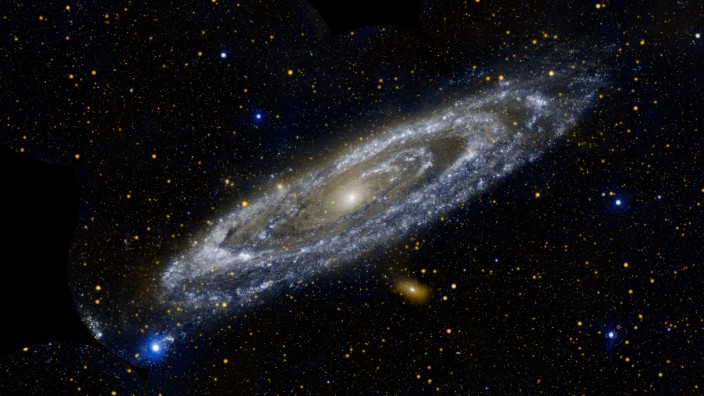
\includegraphics[width=0.7\textwidth]{figures/galaxy.jpg} % Adjust the width and image filename
		\end{figure}
	}
	 
	\vspace{5.1cm}	
	\noindent
	Fach: Physik \noindent\\
	Betreuungsperson: Dr. Andreas Schärer\\
	Abgabetermin: 11.9.2023
	
\end{titlepage}
